\documentclass[sigconf]{acmart}

\usepackage[utf8]{inputenc} %unicode support
\usepackage{hyperref}
\usepackage{graphicx}
% \usepackage{subfig}

% DOI
\acmDOI{10.475/123_4}

% ISBN
\acmISBN{123-4567-24-567/08/06}

%Conference
% \acmConference[WOODSTOCK'97]{ACM Woodstock conference}{July 1997}{El
%   Paso, Texas USA} 
% \acmYear{1997}
% \copyrightyear{2016}
% \acmPrice{15.00}

%%% Begin ...
\begin{document}
\title{Building applications for interactive data exploration in systems biology}

\author[
     addressref={aff1},
     email={bjorn.fjukstad@uit.no}
]{\inits{BF}\fnm{Bjørn} \snm{Fjukstad}}
\author[
   addressref={aff2},                   % id's of addresses, e.g. {aff1,aff2}
  email={vanessadumeaux@gmail.com}   % email address
]{\inits{VD}\fnm{Vanessa} \snm{Dumeaux}}
\author[
   addressref={aff3},                   % id's of addresses, e.g. {aff1,aff2}
  email={karina.standahl.olsen@uit.no}   % email address
]{\inits{KSO}\fnm{Karina Standahl} \snm{Olsen}}
\author[
   addressref={aff3},                   % id's of addresses, e.g. {aff1,aff2}
  email={eiliv.lund@uit.no}   % email address
]{\inits{EL}\fnm{Eiliv} \snm{Lund}}
\author[
   addressref={aff1},                   % id's of addresses, e.g. {aff1,aff2}
   corref={aff1},                       % id of corresponding address, if any
  email={larsab@cs.uit.no}   % email address
]{\inits{LAB}\fnm{Lars Ailo} \snm{Bongo}}

%%%%%%%%%%%%%%%%%%%%%%%%%%%%%%%%%%%%%%%%%%%%%%
%%                                          %%
%% Enter the authors' addresses here        %%
%%                                          %%
%% Repeat \address commands as much as      %%
%% required.                                %%
%%                                          %%
%%%%%%%%%%%%%%%%%%%%%%%%%%%%%%%%%%%%%%%%%%%%%%

\address[id=aff1]{%                           % unique id
  \orgname{Department of Computer Science, UiT – The Arctic University of Tromsø}, % university, etc
  \postcode{9037}                                % post or zip code
  \city{Tromsø},                              % city
  \cny{NO}                                    % country
}
\address[id=aff2]{%                           % unique id
  \orgname{University of ....}, % university, etc
  \postcode{}                                % post or zip code
  \city{},                              % city
  \cny{}                                    % country
}
\address[id=aff3]{%                           % unique id
  \orgname{Department of Community Medicine, UiT – The Arctic University of Tromsø}, % university, etc
  \postcode{9037}                                % post or zip code
  \city{Tromsø},                              % city
  \cny{NO}                                    % country
}
 
\begin{abstractbox}
    \begin{abstract} % abstract, must be under 350 words
        \parttitle{Background} 
            In scientific fields such as systems biology there is a need for
            interactive data exploration tools to enable new insights in the
            fast growing datasets. 
            These tools need to combine advanced statistical analyses, known
            biology from up-to-date databases, and interactive visualizations.  
            To answer specific research questions tools must
            provide specialized user interfaces and visualizations. While these
            are application-specific, the underlying components of a
            data analysis tool can be shared and reused later. 
            Application developers can therefore compose applications of
            reusable services rather than implementing a single monolithic
            application. 
            
        \parttitle{Results} 
            We have designed an approach for developing data exploration
            applications in systems biology that builds on the microservice
            architecture. We use this approach to build applications that
            integrate advanced statistical software and up-to-date information
            from biological databases with modern data visualization libaries. 
            We demonstrate its viability through a web application for exploring
            and comparing transcriptional profiles from blood and tumor samples,
            MIxT Blood-Tumor.
            In addition we have used it to build two other web-applications and
            several command-line tools. 
            With a microservices approach building on software container
            technology we can re-use and share key components between
            application reducing development, deployment and maintenance time. 
            % LAB: noe om performance & noe om code quality?

        \parttitle{Conclusions}  
            Our approach and reference implementation Kvik is open-sourced at
            \url{github.com/fjukstad/kvik}. The web application for exploring
            transcriptional profiles, MIxT, is available at
            \url{mixt-blood-tumor.bci.mcgill.ca} and its source code at 
            \url{github.com/fjukstad/mixt}. 

    \end{abstract}
    
    \begin{keyword}
    % \kwd{Molecular Sequence Analysis}
    \end{keyword}
\end{abstractbox}

 

\keywords{ACM proceedings, \LaTeX, text tagging}
\maketitle

\section*{Introduction}
In recent years the biological community has  generated  an
unprecedented ammount of data. While the cost of data collection has
drastically decreased, data analysis continue to be a larger fraction of the
total experiment cost.\cite{sboner2011real}  An important part of data analysis
includes the time spent by human experts interpreting the results. This calls
for novel methods for building data analysis tools for data exploration and
interpretation. 

In the field of systems biology, data exploration applications need to link
results to relevant prior knowledge. In the later years there has been a
tremendous effort to curate databases with relevant information on genes and
processes. Databases such as the Molecular Signatures Database
(MSigDB)\footnote{\url{software.broadinstitute.org/gsea/msigdb}} and the Kyoto
Encyclopedia of Genes and Genomes (KEGG)\footnote{\url{kegg.jp}} both provide
interfaces to retrieve data that can be used to better the understanding of
data analysis results. 

Several tools for biological data analysis are now available in various
programming languages. These include a wide variety of bioinformatics
methodologies and graphical analysis tools.
In the R statistical programming language developers share software through
repositories such as CRAN\footnote{\url{cran.r-project.org}} or
Bioconductor\footnote{\url{bioconductor.org}}.  In other languages, libraries
for biological bomputation are often availalbe like BioPython\cite{biopython}
and biogo\cite{biogo} for Python or Go, respectively. Projects such as
Galaxy\footnote{\url{galaxyproject.org}} and Common Workflow Language
(CWL)\footnote{\url{commonwl.org}} enable resarchers to build and run
biological data analysis pipelines consisting of a wide range of tools.
Although these framework are tremendously helpful, we need novel approaches to
build applications that integrate high-performance bioinformatics tools with 
specialized user-interfaces and interactive visualizations.

Different programming languages solve different tasks.  For example, new
biological data analysis techniques are quickly realeased in R and its package
repositories; high-performance computer vision tasks are performed in C++ and
OpenCV; and portable user interfaces more easily built in HTML, CSS and
JavaScript.  
Therefore applications that integrate novel statistical
analysis tools, interactive visualizations, and biological databases likely
need to include several components written in different languages. 

A microservice architecture structures an application into small reusable,
loosely coupled parts. These communicate via lightweight programming
language-agnostic protocols such as HTTP, making it possible to write single
applications in multiple programming languages. This way the
most suitable programming language is used for each specific part. To build a
microservice application, developers bundle each service in a container.
Containers are built from configuration files which describe the operating
system, software packages and versions of these. 
This makes reproducing the analyses, database lookups, library versions in an
application a trivial task. The most popular implementation of a software
container is Docker\footnote{\url{docker.com}}, but others such as
Rkt\footnote{\url{coreos.com/rkt}} exist. Initiatives such as
BioContainers\footnote{\url{biocontainers.pro}} now provide containers
pre-installed with different bioinformatics tools. While the enabling technology
is available, the microservices approach is not yet widely adopted in
bioinformatics.\cite{williams2016growing}

From our experience we have identified a set of components and features we
needed to build data exploration applications.

\begin{enumerate}
    \item A low-latency language-independent approach for integrating, or
        embedding, statistical software, such as R, directly in a data
        exploration application. 
    \item Low latency language-independent interface to online reference
        databases in biology that users can query to better understand resulst
        from statistical analyses. 
    \item A simple method for deploying and sharing the components of an
        application between projects. 
\end{enumerate} 


In this paper, we describe a novel approach for building data exploration
applications in systems biology. 
We show that by building applications as a set
of services we can reuse and share its components between applications. 
The key services of a biological data exploration application are i) a compute
service for executing statistical analyses in languages such as R, ii) a
database query service for retrieving information from biological databases, and
iii) the user-facing visualizations and user-interfaces. 
In addition, by packaging the services using container technology they are easy
to deploy, simple to reproduce, and easy to share between projects. 
We have used our approach to build a number of applications, both command-line
and web-based. In this paper we describe how we used our approach to develop
MIxT, a web application for exploring and comparing transcriptional profiles
from blood and tumor samples. 
 
\section*{Related Work}
% LAB: Si heller hvilke områder som er beskrevet nedenfor
In this section we aim to cover some of the existing systems for building
interactive data exploration applications in systems biology. 

% LAB: Integrate med hva?
\subsection*{Integrate Statistical Analyses} 
% LAB: Siden Kvik nå er beskrevet kan teksten ta hensyn til det. Så feks: It offers -> Similary to Kvik, it offers 
OpenCPU is a system for embedded scientific computing and reproducible
research.\cite{opencpu} It offers an HTTP API to the R programming language to
provide an interface with statistical methods. It enables users to make function
calls to any R package and retrieve the results in a wide variety of formats
such as json or pdf. 
Users can chose to host their own R server or use public servers, and OpenCPU
works in a single-user setting within an R session, or a multi-user setting
facilitating multiple parallel requests. This makes OpenCPU suitable
for building a service that can run statistical analyses. 
OpenCPU provides a Javascript library for interfacing with R, as well as Docker
containers for easy installation and OpenCPU has been used to build multiple
applications.\footnote{\url{opencpu.org/apps.html}}.
% LAB: også er det viktig å avslutte med hvorfor vi ikke like godt brukte OpenCPU eller de andre tingene som beskrives her.

Renjin is a JVM-based interpreter for the R programming language.\cite{renjin}
It enables integrating the R interpreter in web
applications. Since it is built on top of the JVM it allows developers to 
% I Java og Scala? 
write
data exploration applications that interact directly with R code, both running on
top of the JVM. Although Renjin supports a large number of CRAN packages it
cannot access any R package (i.e.  any package from BioConductor or CRAN)
% LAB: Forklar hvorfor ting må skrives om (for å gjøre det helt klart)
without modification. This makes the programming effort to use Renjin as an
interface to R higher. 
% LAB: Vil dette gi bedre/dårligere performance?

% LAB: Kanskje ta denne først, siden den er den mest populære (tror jeg)
Shiny is a web application framework for R\footnote{\url{shiny.rstudio.com}}
It allows developers to
build web applications in R without having to have any knowledge about HTML, CSS
or Javascript. 
% LAB: Skrive hvordan og i hva?
Its widget library to provides more advanced Javascript
visualizations such as Leaflet\footnote{\url{leafletjs.com}} for maps or
three.js\footnote{\url{threejs.org}} for WebGL-accellerated
graphics. Developers can choose to host their own web server with the user-built
Shiny Apps, or host them on public servers. Shiny forces users to implement data
exploration applications in R, limiting the functionality to the 
widgets and libraries in Shiny. 
% LAB: Høres ut som du da slipper overhead med put/get, som antageligvis er veldig liten, og at det er vanskeligere å optimlisere enkelt deler

% LAB: Synes SparkR burde nevnes, her eller ett annet sted

% LAB: Denne, SparkR, og ADAM kan kanskje være ett eget delkapittel om parallel execution
\subsubsection*{Biogo} 
\emph{this one is a bit out of place.}

% LAB: Hva slags functionality? (du kan analysere data i de aller fleste språk)
Biogo is a bioinformatics library written in Go. It provides functionality to
analyze genomic and metagenomic datasets in the go programming
language.\cite{Kortschak005033} Using the go programming language the developers
are able to provide high-performance parallel processing in a clean and simple
programming language. 

\subsection*{Visualization frameworks} 
Cytoscape is an open source software platform for visualizing complex
networks and integrating these with any type of attribute
data\cite{shannon2003cytoscape}. It allows for analysis and visualization in the
same platform. Users can add additional features, such as databases connections
or new layouts, through Apps. One such app is cyREST which allows external network
creation and analysis through a REST API\cite{ono2015cyrest}.
To bring the visualization and analysis
capabilities to the web the creators of Cytoscape have developed
Cytoscape.js\footnote{\url{js.cytoscapejs.org}}, a Javascript library to create
interactive graph visualizations. 
% LAB: Ulemper?

Caleydo is a framework for building applications for visualizing and exploring
biomolecular data\cite{cleydo}. Until 2014 it was a standalone tool that needed
to be downloaded, but the Caleydo team are now making the tools web-based. There
have been several applications built using Caleydo: StratomeX for exploring
stratified heterogeneous datasets for disease subtype analysis\cite{stratomex};
Pathfinder for exploring paths in large multivariate graphs\cite{pathfinder};
UpSet to visualize and analyse sets, their intersections and
aggregates\cite{upset}; Entourage and enRoute to explore and visualize
biological pathways \cite{entourage}\cite{enroute}; LineUp to explore rankings
of items based on a set of attributes\cite{lineup}; and Domino for exploring
subsets across multiple tabular datasets\cite{domino}. 

BioJS is an open-source JavaScript framework for biological data
visualization.\cite{gomez2013biojs} It provides a community-driven online
repository with a wide range components for visualizing biological data
contributed by the bioinformatics community. BioJS builds on
node.js\footnote{\url{nodejs.org}} providing both server-side and client-side
libraries. 

% LAB: DB/ provenance related work? Som Galaxy, Pacyderm, CWL, etc

\subsection*{WIP: Biological Databases} 
Maybe some words here on how to get data out of the different biological
databases? 

\subsection*{WIP: Microservices, Docker etc.} 
... 

\subsection*{Kvik and Kvik Pathwys}
We have previously built a system for interactively exploring gene expression
data in context of  biological pathways.\cite{fjukstad2015kvik} Kvik Pathways is
a web application that integrates gene expression data from the Norwegian Women
and Cancer (NOWAC) cohort together with pathway images from the Kyoto
Encyclopedia of Genes and Genomes (KEGG). We used the experience building Kvik
Pathways to completely re-design and re-implement
the R interface in Kvik. From having an R server that can run a set of functions
from an R script, it now has a clean interface to call any function from any R
package, not just retrieving data as a text string but in a wide range of
formats. We also re-built the database interface, which is now a seperate
service. This makes it possible to leverage its caching capabilities to improve
latency. 

 
\section*{Methods} 
In this section we motivate our microservice approach by describing how we
developed a web application for exploring and comparing transcriptional profiles
from blood and tumor samples, called MIxT Blood-Tumor. We describe the process
from initial data analysis to the final application, highlighting the importance
of language-agnostic services to facilitate the use of different tools in
different parts of the application. This is especially important in
interdisciplinary teams where researchers use a wide range of tools. We believe
many system biology data exploration applications are developed similarly and
that they can therefore also benefit from the microservice approach. 

% Bruke MIxT til å fortelle hvordan de forskjellige delene ble gjort og hvordan
% man kan bygge en app uten å gjore alt på nytt igjen, eller hvertfall kunne
% bygge på det man har. 
% 1) les inn data (bioconductor) 
% 2) se på de slå sammen, kanskje enkle vis
% 3) gjøre analyser
% 4) koble resultat opp mot db
% 5) gå gjennom resultatene og db interaktivt.
% 6) del med andre 

\subsection*{Analyzing biological datasets} 
We analyzed profiled RNA in blood and matched tumor from 173 patients in the
Norwegian Women and Cancer (NOWAC) study. Each profile measures the expression
of 16 782 unique genes. 

% BF: Hei LA var dette noe sånn du så for deg? 
We used R and various packages from Bioconductor and CRAN to pre-process and
analyze the gene expression dataset. 
From the initial analyses we built an R package that makes
it possible to share results between researchers within, and outside our group.
To build an application on top of the analyses there are two possibilities: i)
develop a script that generates a static output file (e.g. generate a
html report or CSV files that contain the result data) and build an application
that uses this static data; or ii) use a framework such as Shiny or OpenCPU to
create a dynamic application that interface directly with the R code. To update
an application that builds on top of a static output file
requires manual execution of the output script, while using Shiny or OpenCPU
this task.  

% Ville ikke sagt "we typically". Men heller beskrevet konkret hva som ble gjort
% for MIxT. Generealisering kan gjøres i neste avsnitt der microservice apporach
% blir beskrevet.  Også ville jeg likt å se tall her. Hvor stort er datasettet?
% Hvor lang tid tar det? Er dette i critial path for data exploration eller bare
% pre-processing? 
We typically start off with a messy dataset that needs to go through
several stages of clean-up and preprocessing before we can analyze it.
% Hvordan gjøres dette? Er dette egentlig protptyping, og dermed en slags
% requirements spec for de endelige visualiseringene? Kan dette gjenbrukes eller
% er det mest bruk-og-kast? Hvem gjør dette? 
After the
preprocessing we typically develop some simple visualizations that help discover 
simple patterns in the data. 
% Apply or develop for MIxT?
After this quick dirty data exploration we start to
apply more advanced statistical methods to look for more intricate patterns in
the data.
% Kommer litt overaskende siden det aldri ble sagt hva formålet med dette var :)
% Database lookup for hva?
After this analysis we often end up with genes or lists of genes of
interest that we can use to guide database lookup.
% Hva med non-quirky visualiseringer integrert med database lookup?
% Hva med visualiseringer for andre brukere? Og data?
% Hva med neste verktøy, dvs MIxT for eksempel for methylation + gene
% expression?

% Savner en diskusjon om performance, resource usage, og andre krav til MiXT

% Tror det er enklere å henge med hvis dette blir flettet inn i teksten over
In terms of data analysis code, the preprocessing steps typically consist of
one or more R scripts that we knit \cite{knitr} into PDF reports that we can
revisit later. From these scripts we end up with analysis-ready datasets that
can be shared within the group. The remaining downstream analysis often starts
out in scripts, that are built into R packages with analysis code that can be
shared between researchers. 

\subsection{Kvik micoservices}
% Noe av dette er kanskje allerede i "Building applications"

Based on the development of MiXT and other data exploration tools, we have
generalized our experience into the following design principle guidelines and
microservices provided by the Kvik framework:

Principle 1: language-agnostic (samme har de funnet ut i blant annet Facebook for Thrift)
Principle 2:

Microservice 1: Databases...
Microservice 2: Statistical analyses...

% Også er det viktig å ikke glemme "system aspects" performance, management,
% deployment, etc for disse. Det kn enten forklares her eller senere.

% Det er ikke forklart hvordan ting henger sammen i Kvik, så dette er vanskelig å forstå
With this process in mind, we designed the interface to the R programming
language in Kvik. We want to make it possible to call any function from an R
package and return its results either as plain text, such as comma-separated
tables, or binaries such as images. Enforcing that R code is built into R
packages ensures that the analysis code can be used by power users through an
ordinary R session or in the data exploration application itself. 

\subsection*{Databases} 

Similar to how our analysis process shaped the R interface, it also defined how
we want to build interfaces to online databases. 

% Kan også beskrive hva slags interfaces de eskponerer, hva som er performance
% characteristics, programmerings utforderinger, og tilatt bruk
In its initial state we wanted an interface to interactively query databases
such as KEGG or MSigDB for up-to-date information about genes, gene sets or
biological pathways. This interface should be available within the data
exploration applications to provide valuable metadata, such as gene summaries,
for the researchers exploring results.  

% TODO: Describe the interfaces/API. 
% + abstraksjoner som tar seg av caching og provenance management

% Jeg ser for meg at det er nyttig å kunne si for alle database oppslag noe sånt
% som: read cached value = False, cache result = "session". Dvs alltid les
% nyeste verdi, men cache resultatene for denne session. Kanskje er det også
% andre database-generisk operasjoner som er nyttige abstraksjoner (hent alle
% entries i en liste). Også er det sikkert mulig å pakke disse inn i en
% interface som kan brukes til å implementere database spesifike (KEGG, MsigDB)
% komponenter.


\subsection*{Building applications} 

% Snu om setningene: microservices som lar implemntere i multiple ways
With Kvik there are multiple ways developers can build data
exploration applications. Either bundle analysis and database lookup on a single
computer, or separate computational tasks to more powerful compute clusters to
improve performance. 
In this paper we discuss how to develop applications that follow a
microservices architecture where data analysis and storage is simply a service. 

% Dette er kanskje en av flere microservices?
In Kvik we use R packages as the fundamental building block for data exploration
applications. They provide an interface to data and analyses, and especially in
the field of systems biology, the R programming language provide the largest
collection of data analysis packages. % litt vagt kanskje? 
We discovered that the most sensible way to build applications on top of our
existing code base was to build a system that could interface with our analysis
code directly. In Kvik we built an HTTP interface on top of R that allows users
to call functions and get results using any programming language with an HTTP
library. This allows developers to build data exploration applications in the
programming language that is most suitable, or has the best support, for
presenting that specific data type. 

\subsection*{Statistical analyses}
\emph{Describe how we've designed the interface with R: Build an R-package and
call functions from it, we provide four different output formats to the user
(json, csv, pdf, png),  as well as four different http endpoints (call, get and
rpc).}

% Hva er fordelene med å gjøre det i go?
The R interface in Kvik follows many of the design patterns in OpenCPU. Both
systems interface with R packages using a hybrid state pattern over HTTP. Both
systems provide the same interface to execute analyses and retrieve results.
While OpenCPU is implemented on top of R and Apache, Kvik is implemented from
the ground up in Go. Because of the similarities in the interface to R in Kvik
we provide packages for interfacing with our own R server or OpenCPU R servers
through the \emph{gopencpu} package. 

The R server in Kvik builds on the standard \emph{http} library in Go. On start
it launches a user-defined number of R sessions that execute analyses on demand.
This allows for parallel execution of analyses. We provide a simple FIFO queue
for queuing of requests. The R server also provides the opportunity for users to
cache analysis results to speed up subsequent calls. 

The Kvik R server is suitable for applications where the analysis should be run
on a different server than the web-server hosting the application. If users want
to bundle both the application and R server on the same machine, the \emph{r}
package in Kvik provides this functionality. Although this is possible, we
believe that following a modular approach separating analysis and
application user-interface makes a cleaner and easier to maintain application. 

\subsection*{Databases}
Describe the interface to the databases and what we use it for. Could be
interesting to talk about provenance/caching.

% LAB: her er stedet for alle Go bibliotek og andre lavnivå detlajer
\subsection*{Implementation}

% LAB: Litt usikker på om dette hører til i Results eller Methods
\subsection*{Applications}

% LAB: kort beskrivelse av hva alle apps gjør

% LAB: Figur som viser hva som er felles og ulikt for alle appene. Her bør noe
% være likt ellers har vi bare 3-4 applikasjoner :)

% LAB: mer detaljert beskrivelse av hvordan hver app er implementert med Kvik


 
\section*{Results}
% Jeg tror det er tre spørsmål som kan besvares her:
% 1. Hvor mye enklere/bedre er det å utvikle apps med Kvik microservices?
% 2. Overhead/ improvement for enkelt-microservices. Dvs overhead for de som
% tilbyr noe mer en alternativet (container tilbyr enklere deployment men har en
% overhead på...), og improvement for de som optiamliserer noe (Kvik vs OpenCPU,
% eventuelt begge deler (caching for MsigDB reduserer query tid men har en
% storage overhead)
% 3. Performance analyse av MIxT. Hvor er det overheadene er for en query? Overhead for mange samtidige queries?
%
% Metodologi:
% 1. Kvik-MIxT vs 1000-R-linjer-MIxT? Og kanskje anektdoter som at container
% kunne flyttes til AWS. Eller noe helt annet.
% 2. En av de enklere web apps som er laget før. Eventuelt en benchmark app.
% 3. MIxT operasjoner.
%
We show the viability of the microservices approach in Kvik by describing the
MIxT web application for exploring and comparing
transcriptional profiles from blood and tumor samples. 

% \subsection*{Design} 
We define six data exploration tasks that the web application should help users
perform: 

\textbf{Explore co-expression gene sets in tumor and blood tissue}. We want to
simplify the process of exploring the computed co-expression gene sets, or
modules, through the web-application. The application should 
visualize gene expression patterns together with clinicopathological variables
for each module. In addition we want to enable users to study the underlying
biological functions of each module by including gene set analyses between the
module genes and known gene sets. 

\textbf{Explore co-expression relationships between genes}. Users should be able
to explore the co-expression relationship as a graph visualization. The network
should visualize each gene as a node and a significant co-expression
relationship as an edge.  

\textbf{Explore relationships between modules from each tissue.} Users should be
able to explore the relationship between modules from different tissues. We
provide two different metrics to compare modules, and the web application should
enable users to interactively browse these relationships. In addition to
providing visualizations the compare modules from each tissue, users should also
be able to explore the relationships, but for different breast cancer patient
groups. 

\textbf{Explore relationships between clinical variables and modules.} In
addition to comparing the association between modules from both tissues, users
also have the possibility of exploring the association with a module and a
specific clinical variable. This should also be possible for the different
breast cancer patient group. 

\textbf{Explore association between user-submitted gene lists and computed
modules.} We want to enable users to explore their own gene lists to explore
them in context of
the co-expression gene sets. The web application must handle uploads of gene
lists and compute association between the genelist and the MIxT modules on
demand. 

\textbf{Search for genes or gene lists of intrest}. To facilitate faster lookup
of genes and biological processes, the web application should provide a search
functionality that lets users locate genes or gene lists and show association to
the co-expression gene sets. 

\begin{figure*}[h!]
\centering
\caption{MIxT module overview page. The screenshot show the user interface for
exploring a single module. It consists of three panels. The top left panel
contains the gene expression heatmap. The top right panel contains a table of
the genes found in the module. The bottom panel contains the results of gene
overlap analyses from the module genes and known gene sets from MSigDB.}
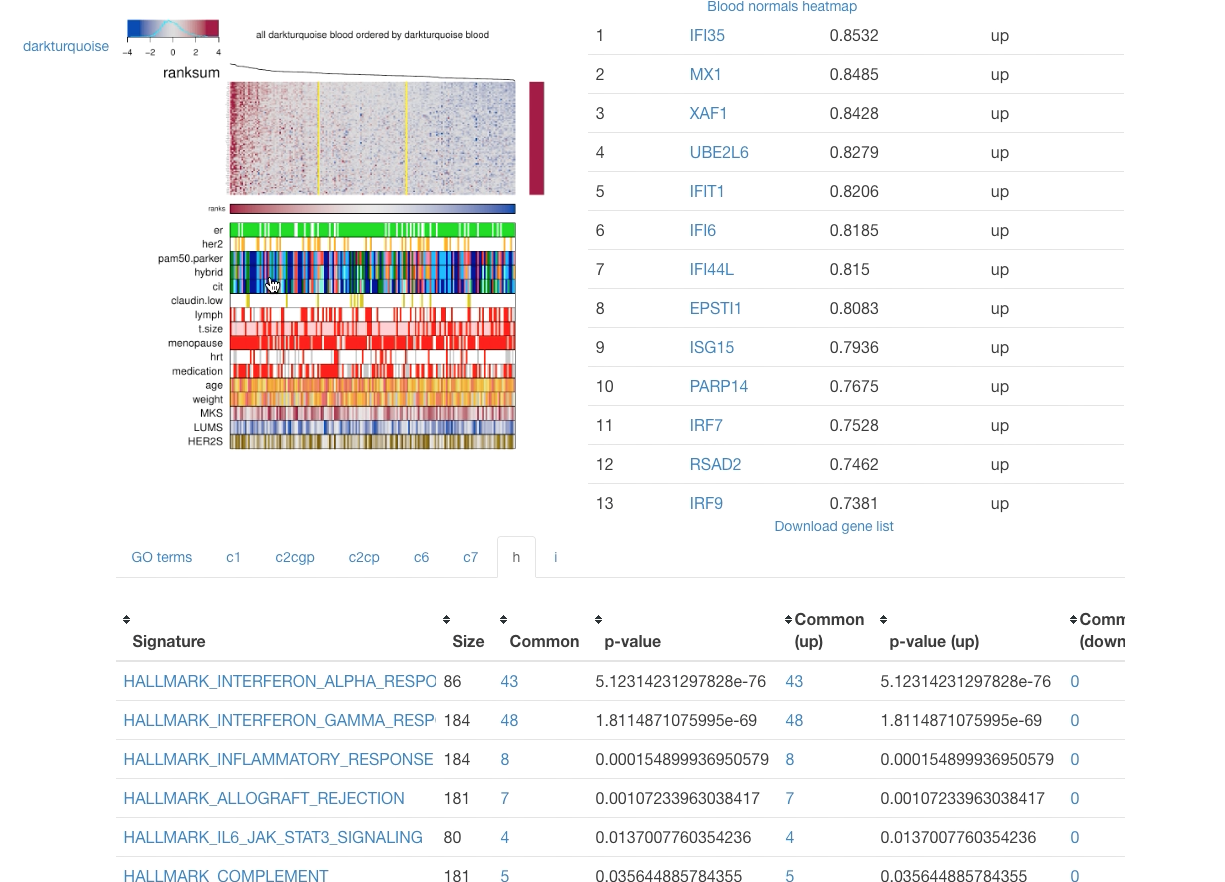
\includegraphics[width=0.8\textwidth]{figures/module.png}
\label{fig_first_case}
\end{figure*} 

From these six analysis tasks we designed and implemented MIxT as a web
application that integrates statistical analyses and information from biological
databases together with interactive visualizations.
The MIxT web application
consists of three services: i) the web application itself containing the
user-interface and visualizations; ii) the compute service performing the MIxT
analyses delivering data to the web application; and iii) the database service
providing up-to-date information from biological databases. Each of these
services run within Docker containers making the process of deploying the
application simple. 
By composing the
application of a set of services we can substitute parts of the application
without re-writing the entire application.
For example if we want to use OpenCPU to interface with data analysis we can do
so by simply exchanging the Kvik compute service with OpenCPU. Both services
communicate over HTTP and their interfaces are the same. 

We structured the MIxT application with a separate view for each analysis task.

To explore the co-expression gene sets we built a view that combines both static
visualizations from R together with interactive tables with gene overlap
analyses. Figure \ref{fig_first_case} shows the web page presented to users when
they access the co-expression gene set 'darkturquoise' from blood. Using the
Kvik compute service we can generate plots on demand and provide users with
high-resolution PDFs or PNG files. 

To explore the co-expression relationship between genes we use an interactive
graph visualization build with Sigmajs\footnote{\url{sigmajs.org}}. We have
built visualization for both tissues, with graph sizes of 2705 nodes and 90 348
edges for the blood network, and 2066 nodes and 50 563 edges for the biopsy
network. The sigmajs visualization library has functionality for generating a
layout for large networks, but we generate this layout server-side to reduce the
computational load on the client. To generate this layout we use the GGally
package\footnote{\url{cran.r-project.org/web/packages/GGally}}. By generating
the network layout using the compute service we relieve the clients.

To visualize relationships between modules from different tissues, or their
relationship to clinical variables we built a heatmap visualization using the 
d3\footnote{\url{d3js.org}} library. Figure \ref{fig_second_case} shows an
example of this heatmap visualization, showing the association between the
clinical variables and the modules from biopsy for all samples.  

\begin{figure}[h!]
\centering
\caption{Heatmap visualization of the association between clinical variables and
the modules in biosy. The visualization is built using the d3 JavaScript
library.} 
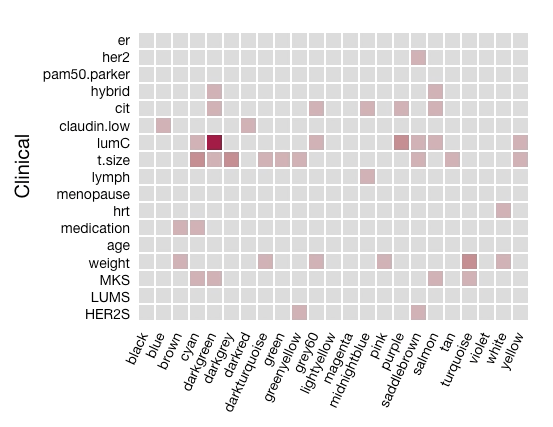
\includegraphics[width=2.5in]{figures/clinical-comp.png}
\label{fig_second_case}
\end{figure} 
 
\section*{WIP: Discussion} 
% Pros/Cons of using a microservice approach. 
% Lessons learned? 

% pros: 
%   lett å dele og gjenbruke 
%   lage en apps med flere språk 
%   slipper én stor app
%   lette klienter 

% cons:
%   kan være vanskelig å monitorere/
%   development time kan være lengre, men det blir bra til slutt
%   krever av dev. kan noe om deploy 

We argue that developing data exploration applications using a microservice
architecture is a viable alternative to the traditional monolithic applications.
By packaging each component of an application in a software container
application developers can reuse and share parts of an application across
research teams and projects. 

Although the partition of components can help break up an application into
manageable parts, there is more overhead with deploying and monitoring these
than a single application. Leslie Lamport's famous quote \emph{You know you have
a distributed system when the crash of a computer you’ve never heard of stops
you from getting any work done.} perfectly describes the possible challenges
application developers face when moving into a microservice architecture.
Monitoring the health of the different services and keeping the services running
is a challenge, but systems such as Kubernetes\footnote{\url{kubernetes.io}}
provide the necessary functionality to manage containerized applications. 


% LAB: foreslår å slå sammen discussion med related work
% The compute service in Kvik follows many of the design patterns in
% OpenCPU. Both systems interface with R packages using a hybrid state pattern
% over HTTP. Both systems provide the same interface to execute analyses and
% retrieve results.  While OpenCPU is implemented on top of R and Apache, Kvik is
% implemented from the ground up in Go. Because of the similarities in the
% interface to R in Kvik we provide packages for interfacing with our own R server
% or OpenCPU R servers through the
% \emph{gopencpu} package.\footnote{\url{github.com/fjukstad/kvik/tree/master/gopencpu}} 


\subsection*{Future work} 
Although we have a first working prototype of the microservices and the MIxT web
application, there are a few points we aim to addresss in the future. 

We have built a database service that provides a sufficient interface for the
MIxT web application. While we have developed the software packages for
interfacing with more databases, these haven't been included in the database
service yet. In future versions we aim to make the database service be a
one-stop interface for all our applications. We also aim to improve the
provenance management within the service, enabling users to retrieve the exact 

One large concern that we haven't addressed in this paper is security. In
particular one security concern that we plan to address in Kvik is the
restrictions on the execution of code in the compute service. We plan to address
this in the next version of the compute service, using methods such as
AppArmor\footnote{\url{wiki.ubuntu.com/AppArmor}} that can restrict a program's
resource access. 

We also aim to explore different avenues for scaling up the compute service.
Since we already interface with R we can use the Sparklyr or SparkR packages
to run analyses on top of Spark. Using Spark as an execution engine for data
anlyses will enable applications to explore even larger datasets. 
 
\section*{WIP: Conclusions}
We have designed an approach for building data exploration applications in
systems biology that builds on a microservice architecture. Using this approach
we have built a web application that leverages this architecture to integrate
statistical analyses, interactive visualizations and data from biological
databases. 

 

\section*{List of abbreviations used}
\section*{Competing interests}
The authors declare that they have no competing interests.
% if your bibliography is in bibtex format, use those commands:
\bibliographystyle{bmc-mathphys} % Style BST file
\bibliography{references} % Bibliography file (usua
\end{document}
